%% GECCO full paper — ACM sigconf, double-blind review build.
%% Every measured result comes from generated/numbers.tex, which
%% scripts/paper_assets.py computes from paper/evidence/. Configuration values and the
%% audit-history figures in Section 6 are quoted from paper/PREREGISTRATION.md and
%% paper/STATUS.md. Do not type result numbers here.
\documentclass[sigconf,review,anonymous]{acmart}

\usepackage{booktabs}
\usepackage{graphicx}
\usepackage{xspace}

% Generated by scripts/paper_assets.py — do not edit.
\newcommand{\ArchDiff}{$+$0.12}
\newcommand{\ArchPholm}{0.286}
\newcommand{\BestAccCart}{0.801}
\newcommand{\BestAccGA}{0.750}
\newcommand{\BudgetMismatch}{0}
\newcommand{\CappedDiff}{$-$4.23}
\newcommand{\CappedKtwoRate}{40\%}
\newcommand{\CappedKtwoWins}{8}
\newcommand{\CappedPholm}{0.114}
\newcommand{\CartDiff}{$-$4.21}
\newcommand{\CartPholm}{0.368}
\newcommand{\DeliveredGA}{10.2}
\newcommand{\DeliveredRS}{5.6}
\newcommand{\FriedmanP}{0.202}
\newcommand{\KoneDiff}{$+$0.66}
\newcommand{\KoneDz}{$+$0.50}
\newcommand{\KoneP}{0.011}
\newcommand{\KonePholm}{0.032}
\newcommand{\KoneWins}{15}
\newcommand{\KtwoRate}{45\%}
\newcommand{\KtwoThreshold}{60\%}
\newcommand{\KtwoWins}{9}
\newcommand{\MeanEvaluations}{2{,}546}
\newcommand{\MedianMaxNodesCart}{32.0}
\newcommand{\MedianMaxNodesGA}{5.4}
\newcommand{\MedianMaxNodesRS}{11.2}
\newcommand{\NDatasets}{20}
\newcommand{\NFoldsFrontier}{30}
\newcommand{\RankArch}{2.70}
\newcommand{\RankCart}{2.25}
\newcommand{\RankGA}{2.15}
\newcommand{\RankRS}{2.90}
\newcommand{\RhoBestGap}{0.85}
\newcommand{\RhoBestGapP}{$<$0.001}
\newcommand{\ViolDatasets}{4}
\newcommand{\ViolDelivered}{1}
\newcommand{\ViolDeliveredOf}{79}
\newcommand{\ViolMax}{27}
\newcommand{\ViolMin}{8}
\newcommand{\ViolRS}{0}


\newcommand{\GA}{GA\xspace}
\newcommand{\RS}{RS\xspace}
\newcommand{\hv}{\ensuremath{\mathrm{HV}}\xspace}

\settopmatter{printacmref=false}
\setcopyright{none}
\acmConference[GECCO '27]{Genetic and Evolutionary Computation Conference}{July 2027}{}

\begin{document}

\title{Evolution Beats Random Search but Not Pruning: A Pre-Registered Test of
Multi-Objective Evolutionary Decision-Tree Induction}

\author{Anonymous Author(s)}
\affiliation{\institution{Anonymous}\country{}}

\begin{abstract}
Multi-objective evolutionary algorithms are routinely proposed for inducing decision
trees that trade accuracy against size, and routinely reported to find smaller trees at
``equivalent'' accuracy to CART. We tested that claim on our own system under a
pre-registered protocol with binding kill criteria: 20 OpenML-CC18 datasets, nested
cross-validation, hypervolume over (test accuracy, node count), a random-search baseline
matched to the \GA's evaluation count exactly, and CART's full cost-complexity pruning
path as the comparator. Two of three hypotheses were decided against us. NSGA-II
recovers a better frontier than budget-matched random sampling of the same tree space
(mean $\Delta\hv$ \KoneDiff, Holm-adjusted $p=\KonePholm$, \KoneWins/\NDatasets{}
datasets), so the evolutionary machinery contributes. But it has the larger hypervolume
than CART's pruning path on only \KtwoRate{} of datasets, below the pre-registered
\KtwoThreshold{} threshold, and the pre-registered accuracy-equivalence test
\KthreeFires. The losses concentrate where accuracy needs large trees: the \GA's
delivered frontiers stop at a median of \MedianMaxNodesGA{} nodes against CART's
\MedianMaxNodesCart. We also report what the audit behind this study found: previously
published figures for this system that no run had produced, and two harness errors, in
opposite directions, each of which reversed a kill-criterion verdict. We argue that
budget-matched random search and full pruning paths should be the default comparators
for evolutionary tree induction.
\end{abstract}

\keywords{decision trees, evolutionary multi-objective optimisation, NSGA-II,
interpretability, benchmarking, pre-registration, negative results}

\maketitle

%% ---------------------------------------------------------------------------
\section{Introduction}

Greedy recursive partitioning~\cite{breiman1984} optimises a split criterion that
decomposes over nodes and controls size afterwards by pruning. Evolutionary tree
induction~\cite{barros2012,kretowski2019,rivera2022} instead scores whole trees, and with a
multi-objective algorithm such as NSGA-II~\cite{deb2002} it returns a set of trees along
the accuracy--size trade-off from one run~\cite{zhao2007}. The standard argument for it
is that a global search over whole trees should find models that greedy induction
misses: as small, or smaller, at the same accuracy.

That argument has two natural baselines that published comparisons often
omit~\cite{freitas2004,barros2012}. The first is \emph{random search over the same tree
space with the same number of fitness evaluations}~\cite{bergstra2012}: without it, a
favourable result cannot be attributed to evolution rather than to the representation,
the fitness or the sampling distribution. The second is CART's \emph{entire}
cost-complexity pruning path rather than one tuned or depth-limited tree: a single CART
tree is one point on a trade-off, and comparing a small evolved tree with it on accuracy
compares two points at different sizes rather than two methods.

This paper reports a test of one such system---ours---against both baselines. It is
also a negative-results paper, for a reason worth stating plainly. The project's public
materials claimed ``46--82\% smaller trees with statistically equivalent accuracy''. An
audit of every public claim against the code found that the headline figures had been
typed into a plotting script as literals, that the remaining ones were stale, that the
``equivalence'' rested on non-significant cross-fold $t$-tests (absence of evidence, and
computed on non-independent folds~\cite{dietterich1998}), and that on the newest real
run the \GA lost to depth-matched CART on 7 of 8 datasets. We withdrew the claims,
fixed three hypotheses and four kill criteria in writing before re-running anything,
and report the outcome whichever way it fell~\cite{nosek2018}.

\paragraph{Contributions.}
\begin{itemize}
\item A pre-registered, budget-matched test of NSGA-II decision-tree induction on
\NDatasets{} OpenML-CC18 datasets. Evolution beats random sampling of the same space
(H3 holds); it does not beat CART's pruning path (H1 rejected); and it does not reach
equivalent accuracy to tuned CART (H2 rejected).
\item A mechanism for the H1 failure: the \GA's frontiers are truncated at small trees,
and its hypervolume deficit against CART tracks the accuracy that only larger trees reach
(Spearman $\rho=\RhoBestGap$, exploratory).
\item An account of two evaluation-harness errors---selection on the test fold, and a
per-fold hypervolume reference point---that each flipped a kill-criterion verdict, in
opposite directions. Both are easy to make and hard to see in aggregate numbers.
\item Sensitivity and exploratory analyses (constraint repair; the optimal sparse-tree
solver GOSDT~\cite{lin2020}) and an open, reproducible harness in which every reported
number is generated from committed run output.
\end{itemize}

%% ---------------------------------------------------------------------------
\section{Related Work}

\paragraph{Evolutionary tree induction.} Barros et al.~\cite{barros2012} survey roughly a
hundred evolutionary decision-tree inducers; Kretowski~\cite{kretowski2019} and Rivera-Lopez
et al.~\cite{rivera2022} cover later global and metaheuristic approaches, and
\texttt{evtree}~\cite{grubinger2014} is a maintained single-objective implementation.
Multi-objective variants optimise accuracy against size with Pareto
selection~\cite{zhao2007}; Freitas~\cite{freitas2004} argued early that Pareto approaches
suit data mining precisely because the trade-off should be presented, not fixed in
advance. Many comparisons in this literature use a handful of UCI datasets, a single CART tree
as the baseline, and no baseline that isolates the contribution of the search operators
from that of the representation; our design targets those three gaps.

\paragraph{Optimal sparse trees.} Exact methods find provably optimal trees under a
sparsity penalty or depth limit: OCT~\cite{bertsimas2017} via mixed-integer programming,
and OSDT~\cite{hu2019}, GOSDT~\cite{lin2020}, DL8.5~\cite{aglin2020} and
MurTree~\cite{demirovic2022} via branch-and-bound and dynamic programming over binarised
features, made practical on continuous data by threshold guessing~\cite{mctavish2022}.
Sweeping the penalty yields a frontier directly comparable to ours. The case for
evolution against them is flexibility, not optimality: arbitrary, non-decomposable
objectives and an anytime answer.

\paragraph{Evaluation methodology.} We follow Dem\v{s}ar~\cite{demsar2006} in treating
datasets as the unit of inference, with Wilcoxon signed-rank tests and Holm
correction~\cite{holm1979}; nested cross-validation to avoid selection
bias~\cite{varma2006,cawley2010}; TOST for equivalence~\cite{schuirmann1987}; and the
Nadeau--Bengio variance correction where folds must be the unit~\cite{nadeau2003}.
Pre-registration~\cite{nosek2018} and variance-aware benchmarking~\cite{bouthillier2021}
respond to the same problems we found in our own earlier claims~\cite{lipton2019}.

\paragraph{Measuring interpretability.} There is no agreed measure of how interpretable a
tree is~\cite{lipton2018,doshivelez2017}. Size- and path-length-based proxies are the most
common~\cite{freitas2014,piltaver2016}; we report only those, and do not claim that any of
them is interpretability~\cite{rudin2019}.

%% ---------------------------------------------------------------------------
\section{Method}

\subsection{Representation and operators}
Individuals are binary axis-parallel trees with a maximum depth of 6 and minimum sample
counts per split (8) and per leaf (3). Leaves predict the majority class of the
training rows reaching them. Initial trees grow recursively, stopping at each node with
probability 0.3. Split thresholds are drawn from the midpoints between consecutive
distinct values of the samples reaching the node---CART's candidate set---filtered so
both sides meet the leaf minimum. Variation uses subtree crossover and four mutations:
threshold perturbation snapped to an observed midpoint, feature replacement, subtree
pruning and leaf expansion (weights 0.45/0.25/0.25/0.05).

\subsection{Fitness and selection}
Each training fold is split 80/20 (stratified) into a fitting part and a validation part.
Leaves are fitted on the former and the tree is scored on the latter, so the search never
rewards memorisation. The multi-objective search uses NSGA-II~\cite{deb2002} (DEAP
implementation~\cite{fortin2012}) over (validation accuracy, $-$node count), population
80, 40 generations, crossover 0.72, mutation 0.18. Structurally identical individuals
are removed before environmental selection; without that step, crowding distance does
not separate clones and the front collapsed to copies of one tree within a few
generations. The delivered model set is the final population's first front.

\subsection{Baselines}
\textbf{Random search (\RS).} Draws trees from the \GA's own initialiser, scores them with
the \GA's own fitness and validation split, and keeps a non-dominated archive on those
validation objectives. Its budget is set per fold to the number of evaluations the \GA
actually spent on that fold. Elites carry their fitness across generations, so a \GA run
costs $\mathit{pop}+\mathit{gens}\times(\mathit{pop}-n_\mathit{elite})$ evaluations, not
$\mathit{pop}\times\mathit{gens}$; matching the latter would have underfunded \RS{} by
about 9\%. \textbf{Archived \GA.} Because \RS{} can only deliver an archive, the \GA was
also run delivering its archive over every candidate it scored, as a control for that
bookkeeping difference. \textbf{CART ccp path.} Scikit-learn CART~\cite{pedregosa2011}
with the same sample minimums, fitted at up to 12 values spread along its
cost-complexity pruning path---a frontier obtained with no search at all. As
pre-registered, the path is not depth-limited, whereas the \GA cannot exceed depth 6;
Section~\ref{sec:k2} also reports a depth-capped path.

\subsection{Frontier metric}
Every delivered model is scored once on the held-out test fold; each method's point set
is filtered for dominance in (test accuracy, node count), and its hypervolume is the
area it dominates up to a reference point of accuracy 0 and one node more than the
largest tree any method produced on that dataset~\cite{zitzler1999}. The reference is
fixed per dataset, not per fold (Section~\ref{sec:audit}). Dominance filtering happens
after scoring and selects nothing: every method delivers a set chosen without test
labels. For display we divide hypervolume by the reference node count, giving an area
fraction comparable across datasets; all tests use the raw values.

%% ---------------------------------------------------------------------------
\section{Pre-Registered Protocol}

The hypotheses, datasets, statistics and kill criteria were written down before any
re-run; deviations were recorded, with their expected direction, before the results
they affect were computed.

\begin{description}
\item[H1] The \GA frontier dominates CART's pruning-path frontier by hypervolume on a
majority of datasets.
\item[H2] Held-out accuracy of the \GA's selected tree is equivalent to inner-CV-tuned
CART within $\pm$2 accuracy points (TOST).
\item[H3] The \GA's hypervolume exceeds budget-matched random search's.
\end{description}

\textbf{Kill criteria.} K1: if \RS{} matches the \GA (Wilcoxon over datasets,
$\alpha=0.05$), the evolutionary machinery contributes nothing; publish the software
only. K2: if the \GA has the larger hypervolume than CART on fewer than
\KtwoThreshold{} of datasets, H1 is rejected, and may not be softened to ``competitive on
some datasets''. K3: if the \GA loses more than 2 points to tuned CART on more than
30\% of datasets, no equivalence claim is made. K4: the composite ``interpretability''
score used inside the fitness may not appear as an outcome.

\textbf{Datasets.} All OpenML-CC18~\cite{bischl2021,vanschoren2014} classification tasks
with 500--1500 rows, at most about 50 features and a smallest class of at least 40:
exactly \NDatasets{} datasets, selected by rule before any run. The frequently used
\emph{iris}, \emph{wine} and \emph{breast cancer} sets are excluded as saturated.

\textbf{Evaluation.} Outer $10\times3$ repeated stratified CV for the frontier run
(\NFoldsFrontier{} folds per dataset); per-fold seeds derived from (dataset, fold,
method). The point-estimate run (H2/K3) tunes every method by inner 5-fold CV---the
\GA and \RS{} over accuracy weighting $\{0.5,0.7,0.9\}\times$ depth $\{4,6,8\}$, CART
over depth and $\alpha$ on its pruning path---and, as a recorded deviation for compute,
uses $10\times1$ outer CV. Complexity is reported as nodes, leaves, mean decision-path
length (over training samples) and distinct features used.

\textbf{Deviations.} Recorded before use: (i) midpoint thresholds, for both searchers;
it was measured beforehand to help \RS{} more than the \GA, i.e.\ to make K1 harder;
(ii) validation-split fitness, for both searchers; (iii) the corrected budget formula
above; (iv) $10\times1$ outer CV for K3; (v) a loader fix for a pandas-version change
that re-encoded two datasets, after which all \NDatasets{} datasets reproduce the
committed CART frontiers exactly; (vi) constraint repair (Section~\ref{sec:repair}),
written after K1/K2 were known and therefore reported only as sensitivity.

%% ---------------------------------------------------------------------------
\section{Results}

\subsection{K1: evolution beats random sampling}

Budgets matched on all folds (\BudgetMismatch{} unequal; mean \MeanEvaluations{}
evaluations per fit). The \GA's hypervolume exceeds budget-matched \RS's by
\KoneDiff{} on average ($p=\KoneP$, Holm $p=\KonePholm$, $d_z=\KoneDz$), on
\KoneWins{} of \NDatasets{} datasets (Figure~\ref{fig:hvdiff}). K1 is not triggered. The
archived-\GA{} control is indistinguishable from the standard \GA{} (\ArchDiff, Holm
$p=\ArchPholm$), so the advantage is not an artefact of delivering a final population
rather than an archive. The four-method Friedman test is not significant ($p=\FriedmanP$;
mean ranks \GA{} \RankGA, CART \RankCart, archived \GA{} \RankArch, \RS{} \RankRS), so no
Nemenyi post-hoc is licensed; K1 is defined on the pairwise test, which has more power
here because two of the four methods are near-duplicates.

\begin{figure}
  \centering
  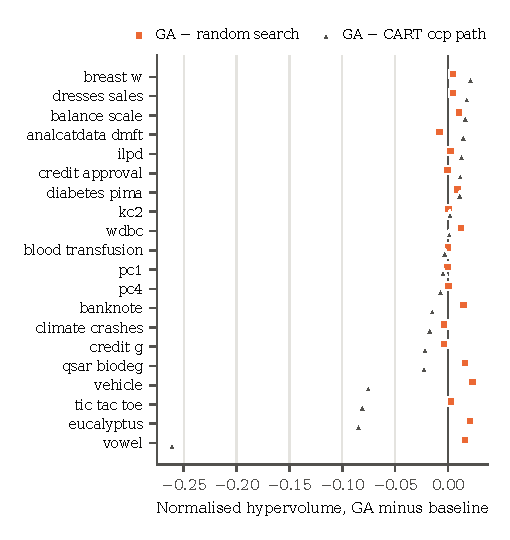
\includegraphics[width=\columnwidth]{generated/fig_hv_diff.pdf}
  \caption{Per-dataset difference in normalised hypervolume between the \GA and each
  baseline (mean over \NFoldsFrontier{} outer folds). Right of zero favours the \GA.
  Datasets sorted by the CART difference.}
  \label{fig:hvdiff}
\end{figure}

\subsection{K2: evolution does not beat pruning}
\label{sec:k2}

The \GA has the larger mean hypervolume than CART's pruning path on \KtwoWins{} of
\NDatasets{} datasets (\KtwoRate), below the \KtwoThreshold{} threshold: \textbf{H1 is
rejected}. The mean difference is \CartDiff{} (Holm $p=\CartPholm$). The depth asymmetry
does not explain this: against CART's path re-derived with the \GA's depth cap on the same
folds and seeds (exploratory), the \GA wins on \CappedKtwoWins{} of \NDatasets{} datasets
(\CappedKtwoRate). Table~\ref{tab:hv}
and Figure~\ref{fig:hvdiff} show the pattern: the \GA wins narrowly on the datasets where
small trees are near-optimal, and loses heavily on \emph{vowel}, \emph{eucalyptus},
\emph{tic-tac-toe} and \emph{vehicle}, where accuracy keeps rising with size.

\emph{Exploratory, post hoc.} The \GA's delivered frontiers are truncated. The largest
tree on its test front has a median of \MedianMaxNodesGA{} nodes across datasets, against
\MedianMaxNodesRS{} for \RS{} and \MedianMaxNodesCart{} for CART, and its best test accuracy
averages \BestAccGA{} against CART's \BestAccCart. Across datasets the hypervolume deficit
to CART is almost entirely explained by that best-accuracy gap (Spearman
$\rho=\RhoBestGap$, $p=\RhoBestGapP$). Figure~\ref{fig:frontiers} shows one fold of each
kind. Where the \GA's front exists it is often at or above CART's; it rarely extends to
the region where the large trees are.

\emph{Exploratory ablation.} To test candidate causes we changed one thing at a time on the
first 10 folds of the \DiagDatasets{} datasets where the \GA loses most, with the committed
\GA as a control arm that reproduces the original fronts exactly. Scoring fitness on the
fitting data instead of a validation split (so that a larger tree need not prove itself on
about a hundred held-out rows) closes \DiagResubClosed\% of the normalised-hypervolume gap to
CART on average. Doubling population and generations closes \DiagBudgetClosed\%. Removing the
bias toward small trees---seeding full-depth trees and swapping the expand and prune
mutation weights---closes \DiagGrowClosed\%, i.e.\ nothing. Under every variant the
largest delivered tree stays between \DiagResubMaxLow{} and \DiagGrowMaxHigh{} nodes against
CART's \DiagCartMaxLow--\DiagCartMaxHigh. The truncation is therefore not an initialisation
artefact; held-out selection and search budget each account for part of it, and most of it
is left unexplained by these three factors. CART's path delivers its large trees without
having to justify them on held-out data, and without searching for them.

\begin{figure}
  \centering
  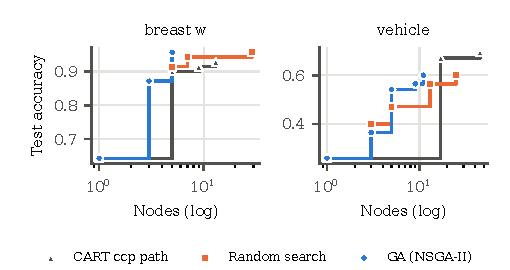
\includegraphics[width=\columnwidth]{generated/fig_frontiers.pdf}
  \caption{Test-fold frontiers for outer fold 1 of a dataset the \GA wins
  (\emph{breast-w}) and one it loses (\emph{vehicle}).}
  \label{fig:frontiers}
\end{figure}

\begin{table}
  \caption{Mean normalised hypervolume per dataset (higher is better; best in bold) and
  the mean node count of the largest tree on the \GA's and CART's test fronts.}
  \label{tab:hv}
  \footnotesize
  \setlength{\tabcolsep}{3pt}
  \begin{tabular}{lrrrrrr}
\toprule
Dataset & GA & RS & CART & GOSDT & \multicolumn{2}{c}{Largest tree} \\
 &  &  &  &  & GA & CART \\
\midrule
analcatdata\_dmft & 0.237 & \textbf{0.245} & 0.223 & 0.228 & 6 & 94 \\
balance\_scale & \textbf{0.749} & 0.738 & 0.732 & 0.704 & 13 & 39 \\
banknote & 0.894 & 0.879 & \textbf{0.909} & 0.890 & 13 & 29 \\
blood\_transfusion & 0.782 & 0.781 & \textbf{0.784} & 0.775 & 6 & 32 \\
breast\_w & \textbf{0.906} & 0.901 & 0.884 & 0.861 & 5 & 13 \\
climate\_crashes & 0.892 & 0.896 & \textbf{0.910} & 0.895 & 2 & 10 \\
credit\_approval & 0.840 & \textbf{0.840} & 0.828 & 0.780 & 4 & 22 \\
credit\_g & 0.723 & 0.727 & \textbf{0.744} & 0.729 & 5 & 48 \\
diabetes\_pima & 0.744 & 0.734 & 0.732 & \textbf{0.758} & 6 & 32 \\
dresses\_sales & \textbf{0.620} & 0.615 & 0.602 & 0.602 & 5 & 36 \\
eucalyptus & 0.521 & 0.500 & \textbf{0.606} & 0.509 & 12 & 63 \\
ilpd & \textbf{0.723} & 0.721 & 0.710 & 0.709 & 4 & 13 \\
kc2 & 0.827 & 0.826 & 0.825 & \textbf{0.838} & 3 & 13 \\
pc1 & 0.919 & 0.919 & \textbf{0.924} & 0.921 & 2 & 16 \\
pc4 & 0.887 & 0.886 & \textbf{0.893} & 0.892 & 4 & 23 \\
qsar\_biodeg & 0.789 & 0.773 & \textbf{0.812} & -- & 9 & 45 \\
tic\_tac\_toe & 0.744 & 0.740 & \textbf{0.825} & 0.800 & 10 & 118 \\
vehicle & 0.594 & 0.570 & \textbf{0.669} & 0.603 & 14 & 77 \\
vowel & 0.360 & 0.343 & \textbf{0.621} & 0.399 & 24 & 155 \\
wdbc & \textbf{0.899} & 0.886 & 0.898 & 0.829 & 5 & 11 \\
\bottomrule
\end{tabular}

\end{table}

\subsection{K3 and H2: accuracy of a single tuned tree}
\label{sec:k3}

With the weighting and depth tuned by inner CV, the single-objective \GA's tree loses
more than 2 points to tuned CART on \KthreePrimary{} of \KthreeN{} datasets, so K3
\KthreeFires{} under the primary reading. The corrected per-dataset TOST fails to
establish equivalence on \KthreeSecondary{} of \KthreeN. Across datasets the mean
difference is \HtwoDiff{} (90\% CI [\HtwoLow, \HtwoHigh], TOST $p=\HtwoP$): the accuracies
are \HtwoVerdict{} within $\pm$2 points, and \textbf{no equivalence claim is made}.
Mean accuracies are \GA{} \AccGA, tuned CART \AccCart, \RS{} \AccRS; the \GA's trees have
\LeavesGA{} leaves (CART \LeavesCart), a mean decision path of \PathGA{} splits (CART
\PathCart) and use \FeaturesGA{} features (CART \FeaturesCart). Figure~\ref{fig:k3}
gives the per-dataset intervals. The smaller trees are real, but they are the product of
the accuracy--size weighting rather than of the search: at the configured weighting a
tree must gain about 8 accuracy points to justify growing from a stump to CART's size.
That is the arithmetic the old ``smaller trees at equivalent accuracy'' claim ignored.

\begin{figure}
  \centering
  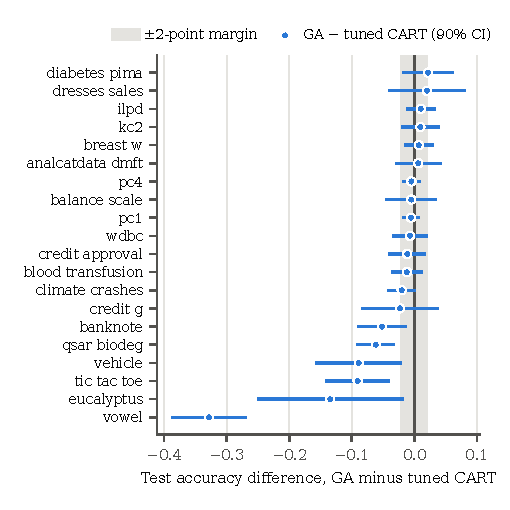
\includegraphics[width=\columnwidth]{generated/fig_k3.pdf}
  \caption{Test-accuracy difference between the tuned \GA tree and tuned CART per
  dataset, with 90\% intervals using the Nadeau--Bengio corrected variance over outer
  folds. The shaded band is the pre-registered $\pm$2-point margin.}
  \label{fig:k3}
\end{figure}

\subsection{Sensitivity: constraint repair}
\label{sec:repair}

The sample-count constraints were enforced only at initialisation. On one fold of each
of \ViolDatasets{} datasets, \ViolMin--\ViolMax\% of the trees NSGA-II evaluated contained a
split the constraints forbid (\ViolRS\% for \RS, whose trees all come from the
initialiser), yet only \ViolDelivered{} of \ViolDeliveredOf{} internal nodes in the delivered
fronts did: the size objective removes dead splits on its own. We added a repair that collapses, top-down, every split
reached by fewer than 8 training rows or leaving fewer than 3 on a side. Re-running the
frontier benchmark with repair on and everything else fixed gives a \GA{}--\RS{}
difference of \RepairKoneDiff{} (Holm $p=\RepairKonePholm$, \RepairKoneWins/\NDatasets{}
datasets) and a CART dominance rate of \RepairKtwoRate. Neither verdict changes. One
secondary result does: with repair, the standard \GA also beats its archived variant
(\RepairArchDiff, Holm $p=\RepairArchPholm$), so the choice between delivering the final
front and the archive is not neutral once dead splits are removed.

\subsection{Exploratory: GOSDT}

GOSDT~\cite{lin2020} with threshold guessing~\cite{mctavish2022}, swept over ten
regularisation values at the same depth limit, run on the first \GosdtFolds{} outer folds
and scored against the same per-dataset reference, has the larger hypervolume than
CART's path on \GosdtBeatsCart{} of \NDatasets{} datasets; the \GA beats GOSDT on
\GABeatsGosdt. It took \GosdtSeconds{} s per fold on average; \GosdtTimeouts{} of
\GosdtFits{} fits hit the 30 s limit and are therefore not certified optimal, and
\GosdtFailures{} returned no model and were dropped from the path (which can only lower
GOSDT's hypervolume). This
comparison was added after K1/K2 were known and decides nothing.

%% ---------------------------------------------------------------------------
\section{What the Audit Found}
\label{sec:audit}

Three findings from the audit behind this study seem more generally useful than the
results themselves.

\paragraph{Published numbers without runs.} The ``46--82\%'' size reduction was spliced from
two dictionaries of literals in a plotting script, and a figure titled ``Statistical
Equivalence to CART'' plotted cross-fold $t$-test $p$-values against a hand-set target of
0.55. The fix was structural rather than editorial: the figure generator now reads only
committed run output and raises an error when there is none, and every number in this
paper is generated from committed CSVs.

\paragraph{Selection on the test fold.} The first frontier run reported K1 triggered, with
\RS{} ahead by a wide margin on 19 of 20 datasets. \RS{} had been returning every tree it
sampled---about 2{,}500 per fold---and the dominance filter then ran on their test
scores: a maximum over thousands of test evaluations that no method could deliver,
since choosing among the candidates needs the test labels. The tell was the delivered
count, 2{,}545 against the \GA's 10. With both searchers archiving on validation
objectives, they deliver \DeliveredGA{} (\GA) and \DeliveredRS{} (\RS) models per fold
and the verdict reverses.

\paragraph{The reference point.} The pre-registration fixes the hypervolume reference per
dataset; the harness computed it per fold. A smaller box favours whichever method has
the lower peak accuracy---here the \GA---and the per-fold version put the CART dominance
rate at 70\%, above the K2 threshold. Computed as specified, it is \KtwoRate. This was found
by reading the implementation against the protocol, not prompted by the result, but it
illustrates why a pre-registration must fix the metric's parameters and not only its
name.

\paragraph{A saved configuration that does not reproduce its run.} Each run saved its
resolved configuration next to its output. The YAML writer sorted keys alphabetically, and
the mutation operator is drawn by position from the ordered weight table, so re-running
from the saved file selected different operators for the same seeds and produced different
fronts. We found this only because an ablation's control arm failed to match the
committed run; the source configuration reproduces it exactly. Serialisation order is part
of the experiment whenever a random draw indexes into a mapping.

\paragraph{Diagnoses that were wrong.} Two pre-run screening measurements (three datasets,
three folds each, so directional only) overturned our own explanations. Midpoint
thresholds were adopted to remove a handicap we believed was suppressing the \GA; they
raised \emph{random search}'s accuracy by 0.012 and lowered the \GA's by 0.003. The \GA
could already reach good thresholds by mutation over generations; \RS{} could not.
Lowering the initial stopping probability to 0 to seed bushier trees made the \GA lose to
\RS{} ($-$0.018): seeded with full-depth trees, \RS{} keeps the large accurate ones
(16.7 leaves) while the \GA, whose mutations favour pruning five to one and whose
single-objective fitness pays for small size, shrinks them back (4.4 leaves). Both
decisions---keep midpoint thresholds, keep the stopping probability at 0.3---were
recorded, with the direction they push K1, before the frontier run.

%% ---------------------------------------------------------------------------
\section{Discussion and Limitations}

The positive result is narrow: over one representation, one fitness and one budget,
NSGA-II beats random sampling of the same space by a medium effect. It is exactly what a
mechanism claim should look like and exactly what a performance claim cannot rest on. The
negative result is also narrow. The \GA was not tuned for the frontier run. The
ablation suggests a larger budget and a less hostile selection scheme each recover part
of the gap, and greedy seeding with CART trees---which would place the large accurate
trees in the population directly---is untested. We did not pursue any of them, because
tuning the \GA after seeing K2 is the forking path the pre-registration exists to close;
they are hypotheses for a new pre-registered study. The datasets are mid-sized
(500--1458 rows, up to 41 features) by design; the K3 run used one outer repeat; the
hypervolume reference depends on the largest tree any method produced; and nothing here
measures whether a human can read these trees faster---size proxies are not
interpretability~\cite{lipton2018,doshivelez2017}.

For evolutionary tree induction generally we draw three recommendations. Report
budget-matched random search over the same representation; it is cheap, and without it
no advantage can be attributed to evolution. Compare frontiers against the full
cost-complexity path, not a single CART tree. And fix the metric's parameters---reference
points, delivered-set rules---in the protocol, because both of our harness errors lived
there and each was large enough to reverse a conclusion.

%% ---------------------------------------------------------------------------
\section{Conclusion}

Evolution earns its place over random sampling in this system, but not over twenty
lines of cost-complexity pruning. We report that as the finding, together with the audit
trail---the withdrawn claims, the two reversed verdicts and the committed data behind
every number---so that the next comparison in this area can start from the baselines
that decided this one.

\section*{Availability}
Code, configuration, pre-registration, deviation log and all run output are in the
project repository (anonymised for review).

\bibliographystyle{ACM-Reference-Format}
\bibliography{refs}

\end{document}
